\documentclass[12pt,letterpaper]{article}
\usepackage{graphicx,textcomp}
\usepackage{natbib}
\usepackage{setspace}
\usepackage{fullpage}
\usepackage{color}
\usepackage[reqno]{amsmath}
\usepackage{amsthm}
\usepackage{fancyvrb}
\usepackage{amssymb,enumerate}
\usepackage[all]{xy}
\usepackage{endnotes}
\usepackage{lscape}
\newtheorem{com}{Comment}
\usepackage{float}
\usepackage{hyperref}
\newtheorem{lem} {Lemma}
\newtheorem{prop}{Proposition}
\newtheorem{thm}{Theorem}
\newtheorem{defn}{Definition}
\newtheorem{cor}{Corollary}
\newtheorem{obs}{Observation}
\usepackage[compact]{titlesec}
\usepackage{dcolumn}
\usepackage{tikz}
\usetikzlibrary{arrows}
\usepackage{multirow}
\usepackage{xcolor}
\newcolumntype{.}{D{.}{.}{-1}}
\newcolumntype{d}[1]{D{.}{.}{#1}}
\definecolor{light-gray}{gray}{0.65}
\usepackage{url}
\usepackage{listings}
\usepackage{color}

\definecolor{codegreen}{rgb}{0,0.6,0}
\definecolor{codegray}{rgb}{0.5,0.5,0.5}
\definecolor{codepurple}{rgb}{0.58,0,0.82}
\definecolor{backcolour}{rgb}{0.95,0.95,0.92}

\lstdefinestyle{mystyle}{
	backgroundcolor=\color{backcolour},   
	commentstyle=\color{codegreen},
	keywordstyle=\color{magenta},
	numberstyle=\tiny\color{codegray},
	stringstyle=\color{codepurple},
	basicstyle=\footnotesize,
	breakatwhitespace=false,         
	breaklines=true,                 
	captionpos=b,                    
	keepspaces=true,                 
	numbers=left,                    
	numbersep=5pt,                  
	showspaces=false,                
	showstringspaces=false,
	showtabs=false,                  
	tabsize=2
}
\lstset{style=mystyle}
\newcommand{\Sref}[1]{Section~\ref{#1}}
\newtheorem{hyp}{Hypothesis}

\title{Problem Set 3}
\date{Due: November 13, 2025}
\author{Applied Stats/Quant Methods 1}


\begin{document}
	\maketitle
	\section*{Instructions}
	\begin{itemize}
		\item Please show your work! You may lose points by simply writing in the answer. If the problem requires you to execute commands in \texttt{R}, please include the code you used to get your answers. Please also include the \texttt{.R} file that contains your code. If you are not sure if work needs to be shown for a particular problem, please ask.
	\item Your homework should be submitted electronically on GitHub.
	\item This problem set is due before 23:59 on Thursday November 13, 2025. No late assignments will be accepted.

	\end{itemize}

		\vspace{.25cm}
	
\noindent In this problem set, you will run several regressions and create an add variable plot (see the lecture slides) in \texttt{R} using the \texttt{incumbents\_subset.csv} dataset. Include all of your code.

	\vspace{.5cm}
\newpage
\section*{Question 1}
\vspace{.25cm}
\noindent We are interested in knowing how the difference in campaign spending between incumbent and challenger affects the incumbent's vote share. 
	\begin{enumerate}
		\item Run a regression where the outcome variable is \texttt{voteshare} and the explanatory variable is \texttt{difflog}.
		
		\textbf{Answer:} 
		A bivariate linear regression was estimated to assess the relationship between incumbent \texttt{voteshare} and the explanatory variable is \texttt{difflog}.
		
			\begin{table}[!htbp] \centering 
				\caption{Regression of Vote Share on Logged Spending Difference} 
				\label{tab:model1} 
				\begin{tabular}{@{\extracolsep{5pt}}lc} 
					\\[-1.8ex]\hline 
					\hline \\[-1.8ex] 
					& \multicolumn{1}{c}{\textit{Dependent variable:}} \\ 
					\cline{2-2} 
					\\[-1.8ex] & voteshare \\ 
					\hline \\[-1.8ex] 
					difflog & 0.042$^{***}$ \\ 
					& (0.001) \\ 
					& \\ 
					Constant & 0.579$^{***}$ \\ 
					& (0.002) \\ 
					& \\ 
					\hline \\[-1.8ex] 
					Observations & 3,193 \\ 
					R$^{2}$ & 0.367 \\ 
					Adjusted R$^{2}$ & 0.367 \\ 
					Residual Std. Error & 0.079 (df = 3191) \\ 
					F Statistic & 1,852.791$^{***}$ (df = 1; 3191) \\ 
					\hline 
					\hline \\[-1.8ex] 
					\textit{Note:}  & \multicolumn{1}{r}{$^{*}$p$<$0.1; $^{**}$p$<$0.05; $^{***}$p$<$0.01} \\ 
				\end{tabular} 
			\end{table}
			\vspace{1em}
			Computed in \texttt{R} as:
			\lstinputlisting[language=R, firstline=36, lastline=46]{PS03_JL.R} 
			\newpage
		
		\item Make a scatterplot of the two variables and add the regression line. 
		
		\textbf{Answer:} 
		A scatterplot was generated to visualise the relationship between incumbent \texttt{voteshare} and \texttt{difflog}, with a fitted regression line overlaid to illustrate the model's linear trend.
		
		\begin{figure}[ht]
			\centering
			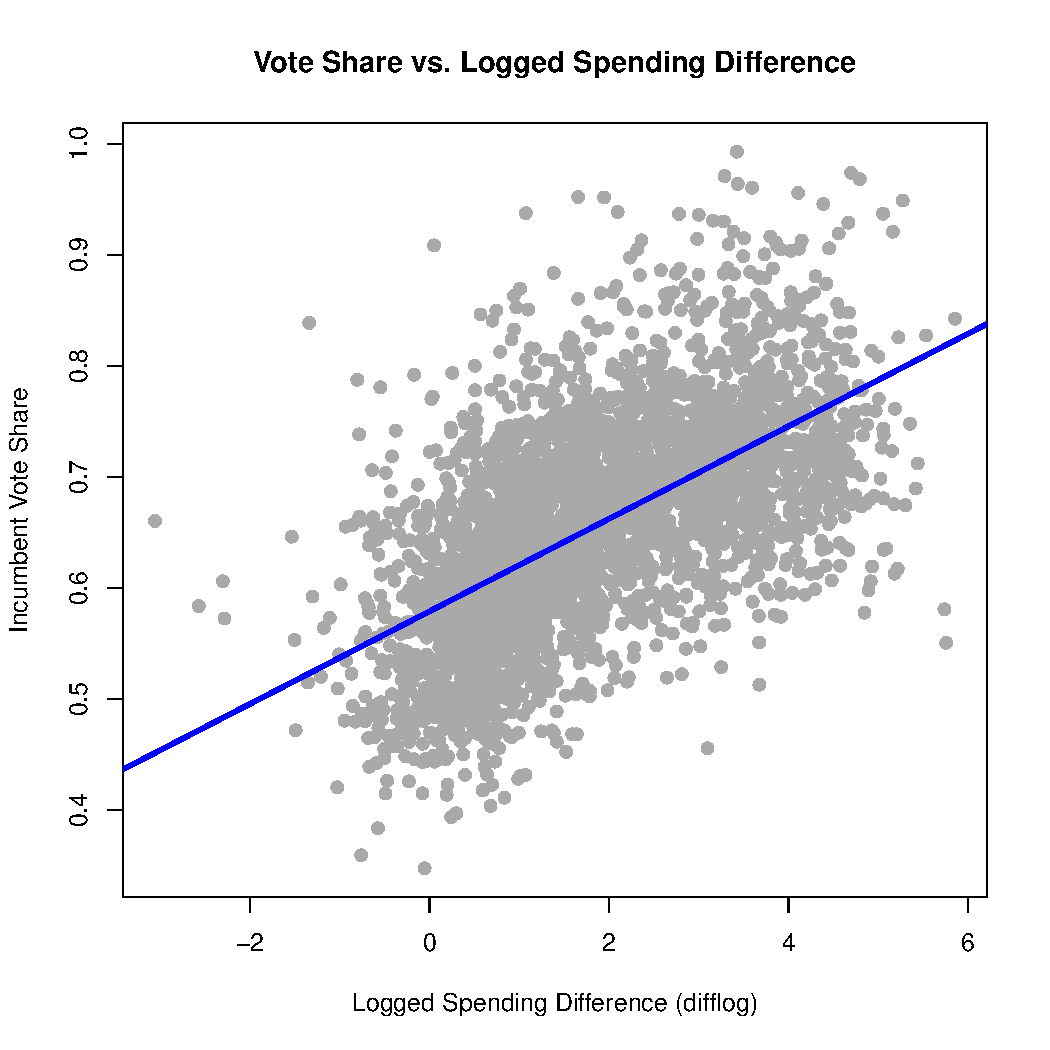
\includegraphics[width=0.7\textwidth]{scatterplot_model1.pdf}  
			\caption{Scatterplot of incumbent vote share vs. logged spending difference}
			\label{fig:scatterplot}
		\end{figure}
		\vspace{1em}
		Computed in \texttt{R} as:
		\lstinputlisting[language=R, firstline=48, lastline=57]{PS03_JL.R} 
		\newpage
			
		\item Save the residuals of the model in a separate object.
		
		\textbf{Answer:} 
		The residuals represent the portion of variation in incumbent \texttt{voteshare} that is not explained by \texttt{difflog}, capturing individual deviations from the model’s predicted values. The residuals from the fitted regression model were saved into a separate object.
		
		\vspace{1em}
		Computed in \texttt{R} as:
		\lstinputlisting[language=R, firstline=58, lastline=60]{PS03_JL.R} 
		\vspace{1.5cm}
		\item Write the prediction equation.
		
		\textbf{Answer:}  The prediction equation indicates that for each one-unit increase in the logged spending difference favoring the incumbent, their expected vote share increases by approximately 4.2 percentage points. The prediction equation reads as follows.
		\[
		\widehat{\texttt{voteshare}} = 0.579 + 0.042 \cdot \texttt{difflog}
		\]
		
		
		
	\end{enumerate}
	
\newpage

\section*{Question 2}
\noindent We are interested in knowing how the difference between incumbent and challenger's spending and the vote share of the presidential candidate of the incumbent's party are related.	\vspace{.25cm}
	\begin{enumerate}
		\item Run a regression where the outcome variable is \texttt{presvote} and the explanatory variable is \texttt{difflog}.
		
		\textbf{Answer:} 
		A bivariate linear regression was estimated to assess the relationship between \texttt{presvote} and the explanatory variable is \texttt{difflog}.
		
		\begin{table}[!htbp] \centering 
			\caption{Regression of Presidential Vote Share on Logged Spending Difference} 
			\label{tab:model2} 
			\begin{tabular}{@{\extracolsep{5pt}}lc} 
				\\[-1.8ex]\hline 
				\hline \\[-1.8ex] 
				& \multicolumn{1}{c}{\textit{Dependent variable:}} \\ 
				\cline{2-2} 
				\\[-1.8ex] & presvote \\ 
				\hline \\[-1.8ex] 
				difflog & 0.024$^{***}$ \\ 
				& (0.001) \\ 
				& \\ 
				Constant & 0.508$^{***}$ \\ 
				& (0.003) \\ 
				& \\ 
				\hline \\[-1.8ex] 
				Observations & 3,193 \\ 
				R$^{2}$ & 0.088 \\ 
				Adjusted R$^{2}$ & 0.088 \\ 
				Residual Std. Error & 0.110 (df = 3191) \\ 
				F Statistic & 307.715$^{***}$ (df = 1; 3191) \\ 
				\hline 
				\hline \\[-1.8ex] 
				\textit{Note:}  & \multicolumn{1}{r}{$^{*}$p$<$0.1; $^{**}$p$<$0.05; $^{***}$p$<$0.01} \\ 
			\end{tabular} 
		\end{table} 
		\vspace{1em}
		Computed in \texttt{R} as:
		\lstinputlisting[language=R, firstline=66, lastline=75]{PS03_JL.R} 
		\newpage
		
		\item Make a scatterplot of the two variables and add the regression line. 
		
		\textbf{Answer:} 
		A scatterplot was generated to visualise the relationship between \texttt{presvote} and \texttt{difflog}, with a fitted regression line overlaid to illustrate the model's linear trend.
		
		\begin{figure}[ht]
			\centering
			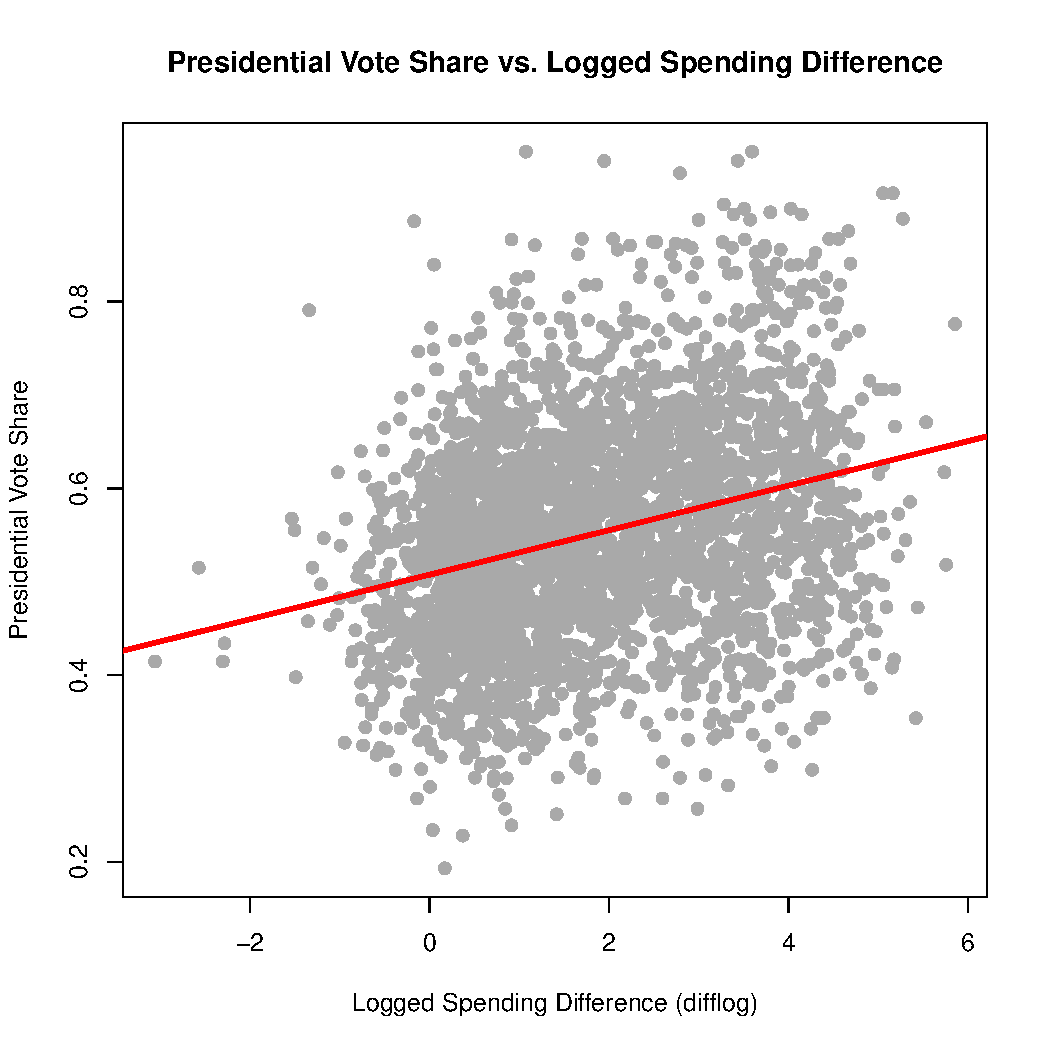
\includegraphics[width=0.7\textwidth]{scatterplot_model2.pdf}  
			\caption{Scatterplot of incumbent vote share vs. logged spending difference}
			\label{fig:scatterplot}
		\end{figure}
		\vspace{1em}
		Computed in \texttt{R} as:
		\lstinputlisting[language=R, firstline=77, lastline=86]{PS03_JL.R} 
		\newpage
		
		\item Save the residuals of the model in a separate object.
		
		\textbf{Answer:} 
		The residuals represent the portion of variation in \texttt{presvote} that is not explained by \texttt{difflog}, capturing individual deviations from the model’s predicted values. The residuals from the fitted regression model were saved into a separate object.
		
		\vspace{1em}
		Computed in \texttt{R} as:
		\lstinputlisting[language=R, firstline=88, lastline=90]{PS03_JL.R} 
		\vspace{1.5cm}
		
		\item Write the prediction equation.
		
		\textbf{Answer:}  The prediction equation suggests that for each one-unit increase in the logged spending difference favoring the incumbent, the expected presidential vote share for the incumbent’s party increases by approximately 2.4 percentage points. The prediction equation reads as follows.
		\[
		\widehat{\texttt{presvote}} = 0.508 + 0.024 \cdot \texttt{difflog}
		\]
	\end{enumerate}
	
	\newpage	
\section*{Question 3}

\noindent We are interested in knowing how the vote share of the presidential candidate of the incumbent's party is associated with the incumbent's electoral success.
	\vspace{.25cm}
	\begin{enumerate}
		\item Run a regression where the outcome variable is \texttt{voteshare} and the explanatory variable is \texttt{presvote}.
		
		\textbf{Answer:} 
		A bivariate linear regression was estimated to assess the relationship between incumbent \texttt{voteshare} and the explanatory variable is \texttt{presvote}.
		\begin{table}[!htbp] \centering 
			\caption{Regression of Incumbent Vote Share on Presidential Vote Share} 
			\label{tab:model3} 
			\begin{tabular}{@{\extracolsep{5pt}}lc} 
				\\[-1.8ex]\hline 
				\hline \\[-1.8ex] 
				& \multicolumn{1}{c}{\textit{Dependent variable:}} \\ 
				\cline{2-2} 
				\\[-1.8ex] & voteshare \\ 
				\hline \\[-1.8ex] 
				presvote & 0.388$^{***}$ \\ 
				& (0.013) \\ 
				& \\ 
				Constant & 0.441$^{***}$ \\ 
				& (0.008) \\ 
				& \\ 
				\hline \\[-1.8ex] 
				Observations & 3,193 \\ 
				R$^{2}$ & 0.206 \\ 
				Adjusted R$^{2}$ & 0.206 \\ 
				Residual Std. Error & 0.088 (df = 3191) \\ 
				F Statistic & 826.950$^{***}$ (df = 1; 3191) \\ 
				\hline 
				\hline \\[-1.8ex] 
				\textit{Note:}  & \multicolumn{1}{r}{$^{*}$p$<$0.1; $^{**}$p$<$0.05; $^{***}$p$<$0.01} \\ 
			\end{tabular} 
		\end{table}
		
		\vspace{1em}
		Computed in \texttt{R} as:
		\lstinputlisting[language=R, firstline=94, lastline=103]{PS03_JL.R} 
		\newpage
		
		\item Make a scatterplot of the two variables and add the regression line. 
		
		\textbf{Answer:} 
		A scatterplot was generated to visualise the relationship between incumbent \texttt{voteshare} and \texttt{presvote}, with a fitted regression line overlaid to illustrate the model's linear trend.
		
		\begin{figure}[ht]
			\centering
			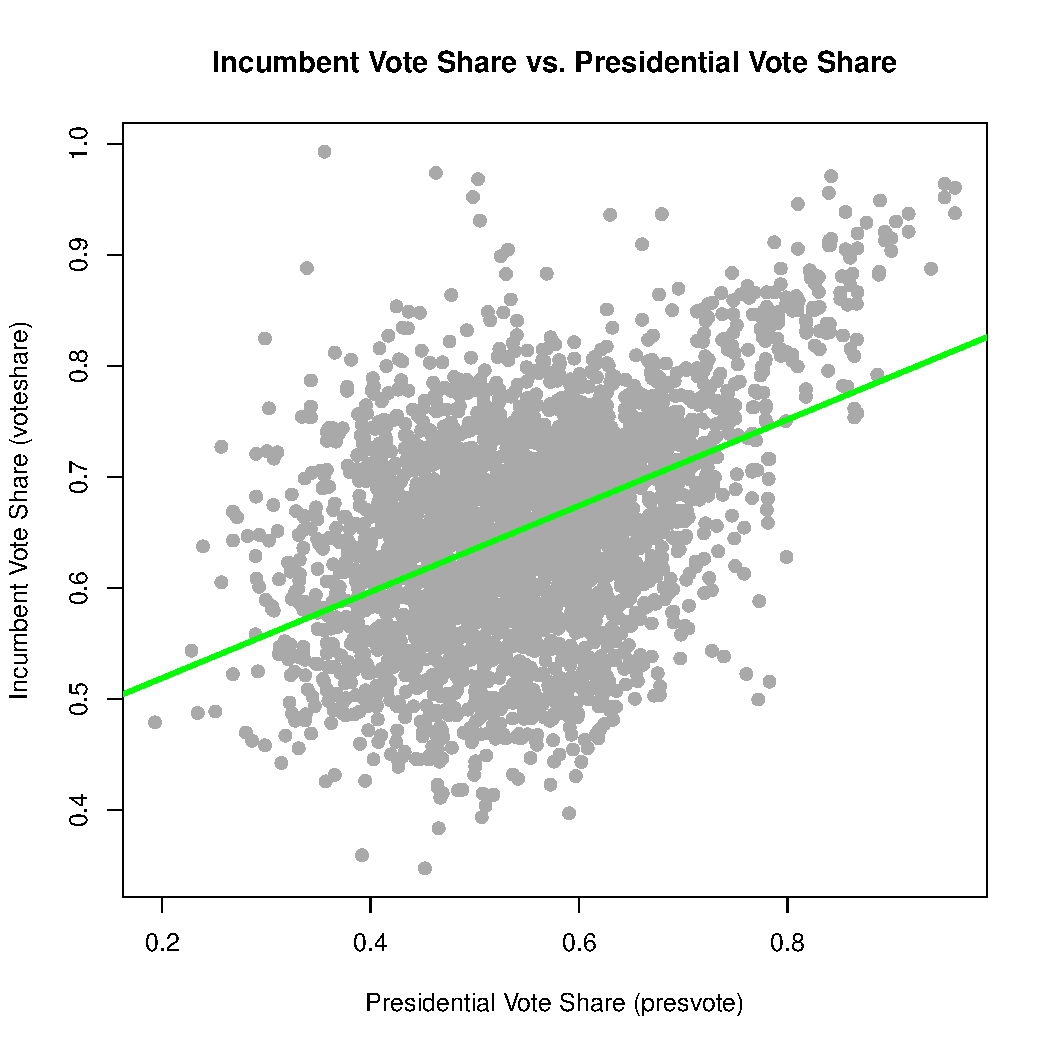
\includegraphics[width=0.7\textwidth]{scatterplot_model3.pdf}  
			\caption{Scatterplot of incumbent vote share vs. presidential vote share of the incumbent's party}
			\label{fig:scatterplot}
		\end{figure}
		\vspace{1em}
		Computed in \texttt{R} as:
		\lstinputlisting[language=R, firstline=105, lastline=113]{PS03_JL.R} 
		\newpage

		\item Write the prediction equation.
		
		\textbf{Answer:}  The prediction equation indicates that for each one percentage point increase in the presidential vote share of the incumbent’s party, the incumbent’s own vote share is expected to increase by approximately 0.388 percentage points. The prediction equation reads as follows.
		\[
		\widehat{\texttt{voteshare}} = 0.441 + 0.388 \cdot \texttt{presvote}
		\]
	\end{enumerate}
	

\newpage	
\section*{Question 4}
\noindent The residuals from part (a) tell us how much of the variation in \texttt{voteshare} is $not$ explained by the difference in spending between incumbent and challenger. The residuals in part (b) tell us how much of the variation in \texttt{presvote} is $not$ explained by the difference in spending between incumbent and challenger in the district.
	\begin{enumerate}
		\item Run a regression where the outcome variable is the residuals from Question 1 and the explanatory variable is the residuals from Question 2.
		
		\textbf{Answer:} 
		To assess the relationship between unexplained variation in incumbent vote share and presidential vote share after accounting for spending differences, a regression was estimated using the residuals from Questions 1 and 2.
		\begin{table}[!htbp] \centering 
			\caption{Regression of Residuals: Incumbent Vote Share on Presidential Vote Share} 
			\label{tab:model4} 
			\begin{tabular}{@{\extracolsep{5pt}}lc} 
				\\[-1.8ex]\hline 
				\hline \\[-1.8ex] 
				& \multicolumn{1}{c}{\textit{Dependent variable:}} \\ 
				\cline{2-2} 
				\\[-1.8ex] & residuals\_model1 \\ 
				\hline \\[-1.8ex] 
				residuals\_model2 & 0.257$^{***}$ \\ 
				& (0.012) \\ 
				& \\ 
				Constant & $-$0.000 \\ 
				& (0.001) \\ 
				& \\ 
				\hline \\[-1.8ex] 
				Observations & 3,193 \\ 
				R$^{2}$ & 0.130 \\ 
				Adjusted R$^{2}$ & 0.130 \\ 
				Residual Std. Error & 0.073 (df = 3191) \\ 
				F Statistic & 476.975$^{***}$ (df = 1; 3191) \\ 
				\hline 
				\hline \\[-1.8ex] 
				\textit{Note:}  & \multicolumn{1}{r}{$^{*}$p$<$0.1; $^{**}$p$<$0.05; $^{***}$p$<$0.01} \\ 
			\end{tabular} 
		\end{table} 
		
		\vspace{1em}
		Computed in \texttt{R} as:
		\lstinputlisting[language=R, firstline=117, lastline=119]{PS03_JL.R} 
		\newpage
		
		\item Make a scatterplot of the two residuals and add the regression line. 
		
		\textbf{Answer:} 
		The scatterplot below visualises the relationship between the residuals from the first two models, highlighting how unexplained variation in presidential vote share corresponds to unexplained variation in incumbent vote share after controlling for spending differences.
		
		\begin{figure}[ht]
			\centering
			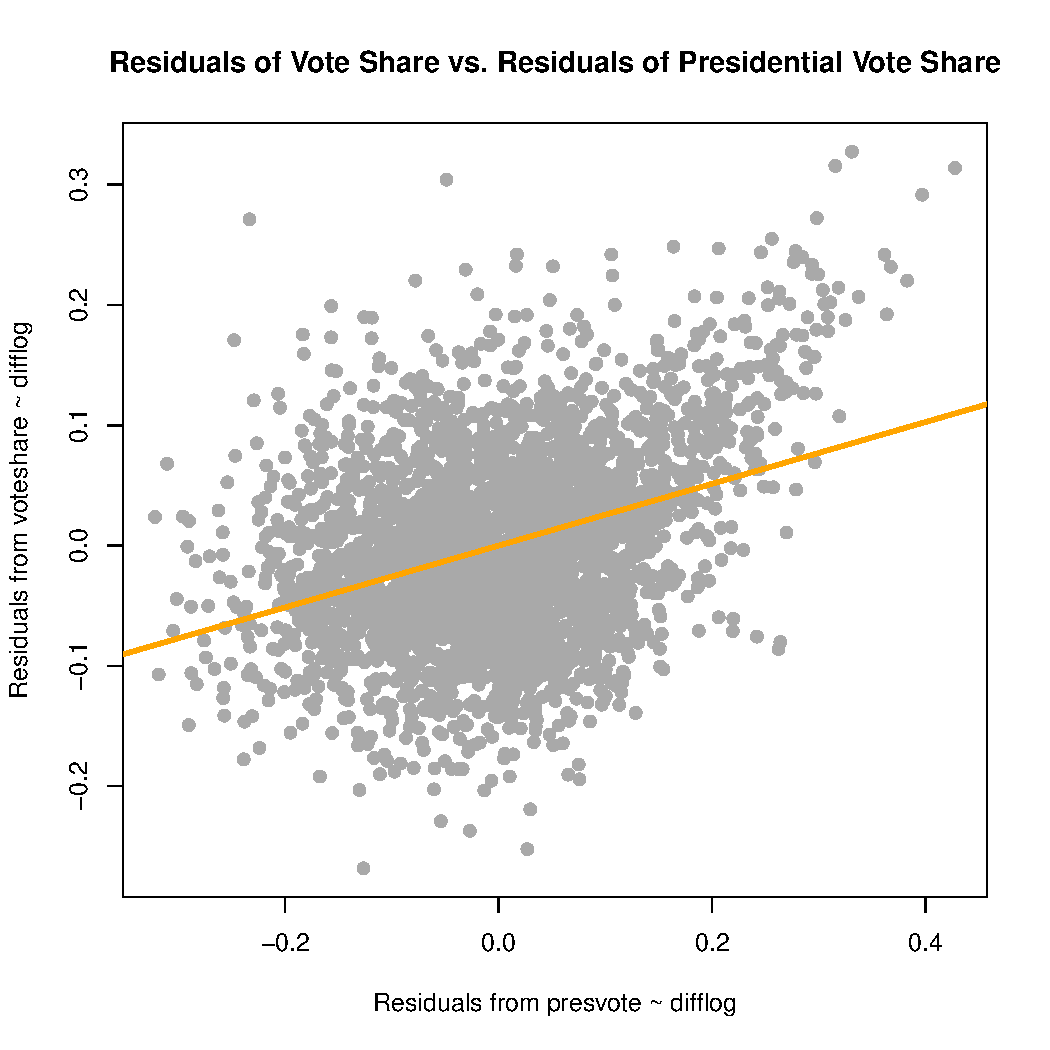
\includegraphics[width=0.7\textwidth]{scatterplot_model4.pdf}  
			\caption{Scatterplot of residuals: incumbent vote share vs. presidential vote share, controlling for spending differences}
			\label{fig:scatterplot}
		\end{figure}
		\vspace{1em}
		Computed in \texttt{R} as:
		\lstinputlisting[language=R, firstline=129, lastline=137]{PS03_JL.R} 
		\newpage
		
		\item Write the prediction equation.
		
		\textbf{Answer:}  The prediction equation indicates that, after controlling for spending differences, a one-unit increase in the residual presidential vote share is associated with a 0.257 unit increase in the residual incumbent vote share. The intercept is necessarily zero because both variables are residuals from prior regressions. By construction, residuals are mean-centered and capture only the variation unexplained by the original models; as a result, their average value---and thus the intercept---is zero. The prediction equation reads as follows.
		\[
		\widehat{\texttt{resid}_{\texttt{voteshare}}} = -0.000 + 0.257 \cdot \texttt{resid}_{\texttt{presvote}}
		\]
	\end{enumerate}
	
	\newpage	

\section*{Question 5}
\noindent What if the incumbent's vote share is affected by both the president's popularity and the difference in spending between incumbent and challenger? 
	\begin{enumerate}
		\item Run a regression where the outcome variable is the incumbent's \texttt{voteshare} and the explanatory variables are \texttt{difflog} and \texttt{presvote}.
		
		\textbf{Answer:} 
		A multiple linear regression was estimated to assess how both \texttt{difflog} and \texttt{presvote} jointly affect the incumbent’s \texttt{voteshare}.
		\begin{table}[!htbp] \centering 
			\caption{Regression of Incumbent Vote Share on Spending Difference and Presidential Vote Share} 
			\label{tab:model5} 
			\begin{tabular}{@{\extracolsep{5pt}}lc} 
				\\[-1.8ex]\hline 
				\hline \\[-1.8ex] 
				& \multicolumn{1}{c}{\textit{Dependent variable:}} \\ 
				\cline{2-2} 
				\\[-1.8ex] & voteshare \\ 
				\hline \\[-1.8ex] 
				difflog & 0.036$^{***}$ \\ 
				& (0.001) \\ 
				& \\ 
				presvote & 0.257$^{***}$ \\ 
				& (0.012) \\ 
				& \\ 
				Constant & 0.449$^{***}$ \\ 
				& (0.006) \\ 
				& \\ 
				\hline \\[-1.8ex] 
				Observations & 3,193 \\ 
				R$^{2}$ & 0.450 \\ 
				Adjusted R$^{2}$ & 0.449 \\ 
				Residual Std. Error & 0.073 (df = 3190) \\ 
				F Statistic & 1,302.947$^{***}$ (df = 2; 3190) \\ 
				\hline 
				\hline \\[-1.8ex] 
				\textit{Note:}  & \multicolumn{1}{r}{$^{*}$p$<$0.1; $^{**}$p$<$0.05; $^{***}$p$<$0.01} \\ 
			\end{tabular} 
		\end{table} 
		
		\vspace{1em}
		Computed in \texttt{R} as:
		\lstinputlisting[language=R, firstline=141, lastline=143]{PS03_JL.R} 
		\newpage
		
		\item Write the prediction equation.
		
		\textbf{Answer:}  The prediction equation below expresses the expected incumbent vote share as a function of both predictors.
		\[
		\widehat{\texttt{voteshare}} = 0.449 + 0.036 \cdot \texttt{difflog} + 0.257 \cdot \texttt{presvote}
		\]
		
		\item What is it in this output that is identical to the output in Question 4? Why do you think this is the case?

		\textbf{Answer:}  
		The coefficient on \texttt{presvote} in this model is exactly the same as the slope from the regression in Question 4. This happens because both models are asking the same underlying question: how does presidential vote share affect incumbent vote share, once we’ve already accounted for the influence of spending differences?
		
		In Question 4, we removed the effect of spending by working with residuals — that is, we looked at what’s left over in both \texttt{voteshare} and \texttt{presvote} after subtracting out the part explained by \texttt{difflog}. Then we ran a regression on those leftover pieces.
		
		In Question 5, we included both \texttt{difflog} and \texttt{presvote} directly in the same model. This gives us the effect of \texttt{presvote} while holding \texttt{difflog} constant — which is mathematically the same as regressing the residuals from Question 4.
		
		So even though the two approaches look different, they’re measuring the same relationship in slightly different ways. That’s why the coefficient on \texttt{presvote} is identical in both cases.
	\end{enumerate}




\end{document}
